\paragraph{ Aufgabe \ref{newinitial}:} Wenn wir bei der Station ''Bellvue'' starten ist die Reihenfolge: $$ \text{\bf{B,KH,HP,KS,N,E/U,P,C,HB,HE}}$$

\paragraph{Aufgabe \ref{directed}:} Wir betrachten jetzt den folgenden Graphen:\\
\begin{figure}[H]
    \centering
    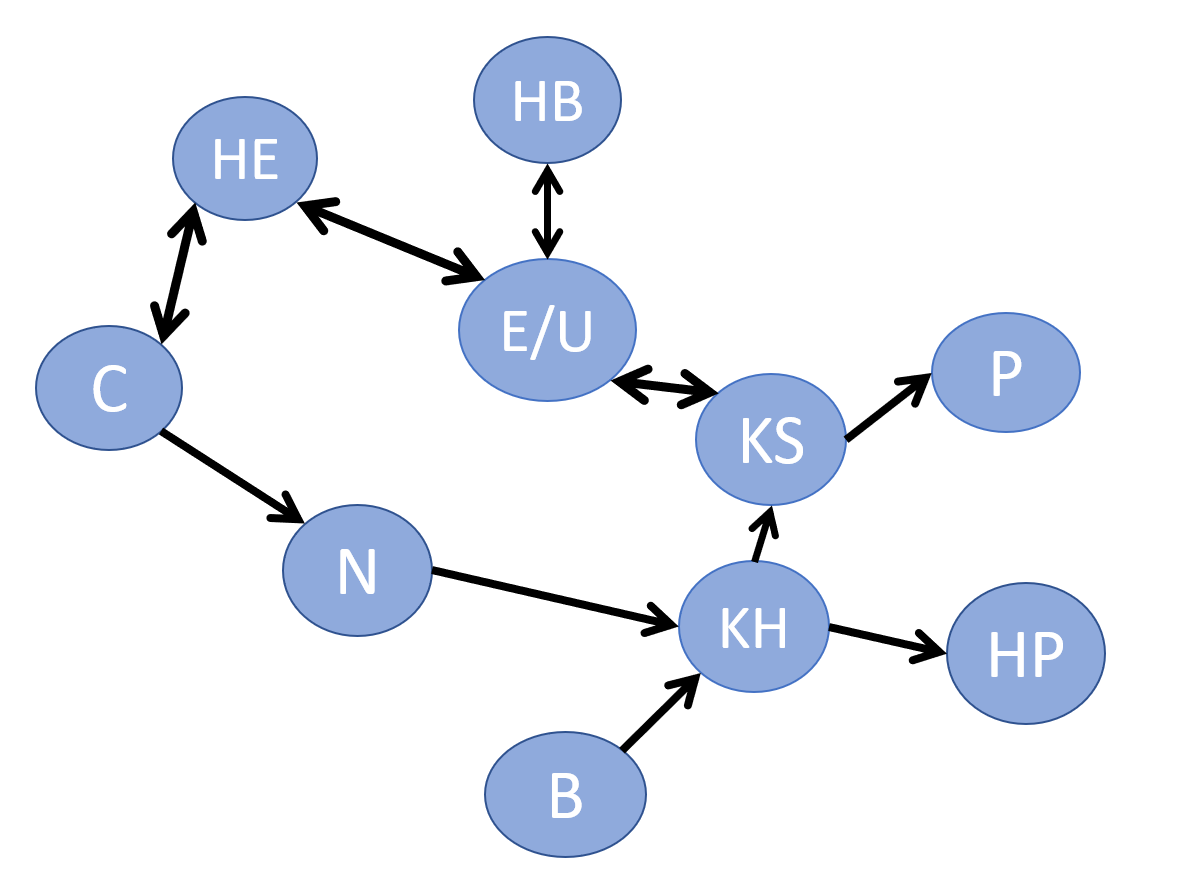
\includegraphics[scale=0.3]{Pictures/directedTram.PNG} 
    \caption{Der gerichtete Graph.}
    \label{fig:my_label}
\end{figure}
Die Reihenfolge in welcher die Breitensuche die Knoten besucht ist:
$$ \text{\bf{B,KH,HP,KS,E/U,P,HB,HE,C,N}}$$

\paragraph{Aufgabe \ref{Wikipedia}}: Wir beginnen die Breitensuche beim Wikipedia-Artikel über die Breitensuche; also bei dem Knoten {\bf{BS}}. Die Reihenfolge ist dann
$$ \text{\bf{BS,D,G,K,L,E,S,U-B,Z,SBZ}}.$$
Bob kann den gewünschten Artikel also finden und wir könen die Breitensuche abbrechen bevor wir den Knoten {\bf{B}} besucht haben.

\paragraph{Aufgabe \ref{ProgFragen}:} Die Liste ''queue'' enthält genau unsere Warteliste, in ''visited'' fügen wir Schritt für Schritt die besuchten Knoten hinzu, so dass wir am Ende mit ''return visited'' die Knoten in der gewünschten Reihenfolge zurückgeben können.

\begin{figure}[H]
    \centering
    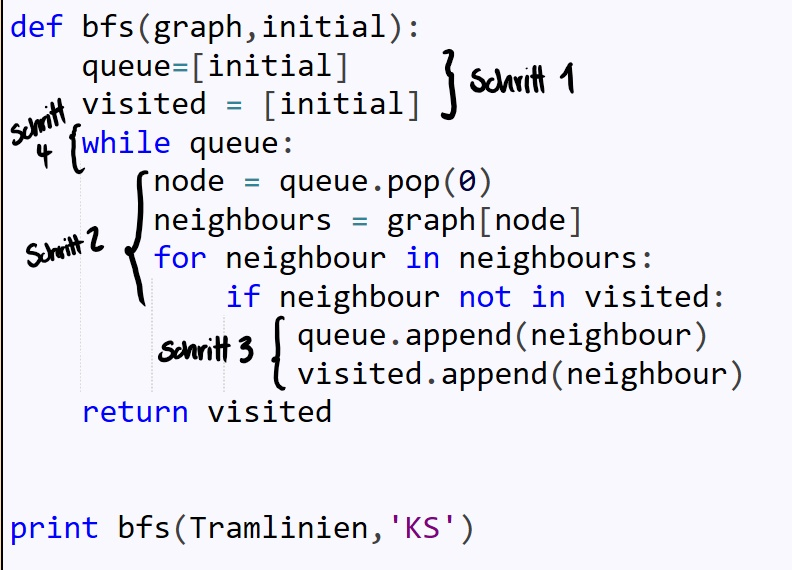
\includegraphics[scale=0.3]{Pictures/Loesung24.jpg}
    \caption{Die 4 Schritte des Algorithmus im Programm}
    \label{fig:ProgLoes}
\end{figure}

\paragraph{Aufgabe \ref{WikiProgAufg}:} Wir implementieren den Graphen der Wikipedia-Artikel in der ''Liste der Nachbarn''-Darstellung und passen das Programm an (Abbildung \ref{fig:my_Prog2Loes}). Falls der Start- und der Zielknoten gleich sind können wir die Suche sofort abbrechen. Ansonsten überprüfen wir jeweils nachdem wir einen Nachabrn als besucht markiert haben, ob dieser der gesuchte Knoten ist. Fall ja können wir die for-Schleife mit break beenden. Damit auch die while-Schleife endet leeren wir noch die Warteliste.

\begin{figure}[H]
    \centering
    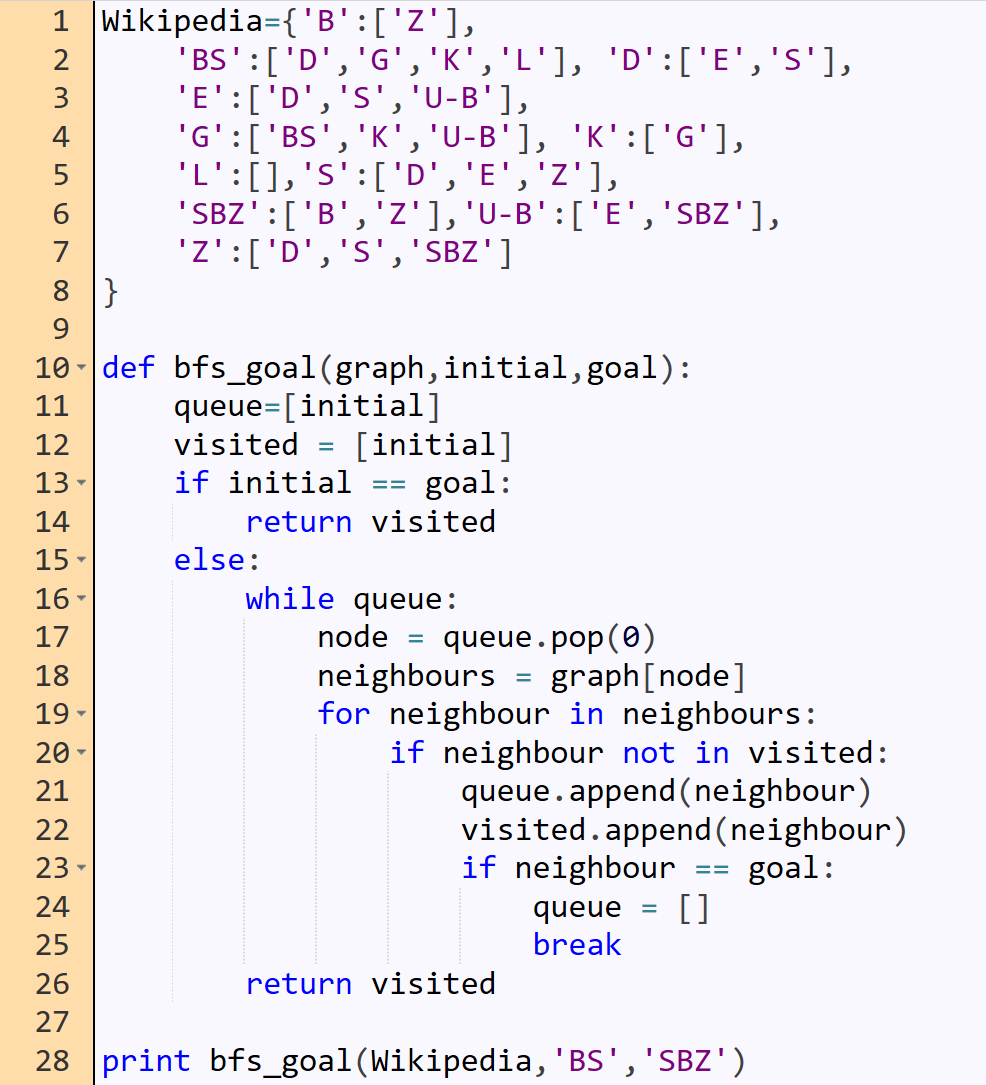
\includegraphics[scale=0.6]{Pictures/WikiProgLoes.PNG}
    \caption{Das Programm mit Zielknoten als Input und einer Abbruchsbedingung}
    \label{fig:my_Prog2Loes}
\end{figure}

\paragraph{Lernaufgabe} 
\begin{enumerate}
    \item Als Knoten nehmen wir alle Menschen. Wir verbinden je zwei Knoten wenn einer ein direkter Nachkomme vom anderen ist. Der Graph stellt also einfach einen Stammbaum dar.
    \item Sie können ''print bfs\_goal (Familien,'Alice','Bob')'' aufrufen. Falls bei der Ausgabe an letzter Stelle 'Bob' steht so haben sie eine gemeinsame Ur-ur-ur-ur-Grossmutter. Wenn die Breitensuche 'Bob' nicht findet, so sind Alice und Bob nicht so nahe verwandt.
    \item der gleichen Zusammenhangskomponente.
    \item Das angepasste Programm:
    \begin{figure}[H]
        \centering
        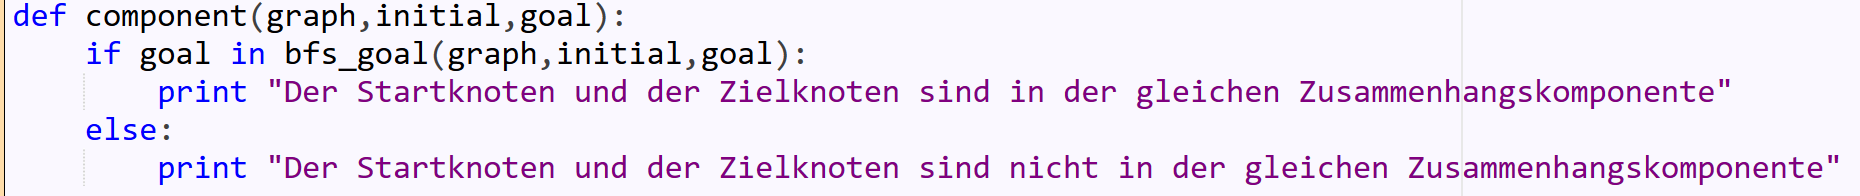
\includegraphics[scale=0.4]{Pictures/components.PNG}
        \caption{Wir rufen bfs\_goal auf und prüfen ob es den Zielknoten finden konnte.}
        \label{fig:my_components}
    \end{figure}
\end{enumerate}

\paragraph{Kontrollfragen}
\begin{enumerate}
    \item -
    \item - 
    \item Die Aussage von David ist falsch. Wir prüfen immer ob wir einen Knoten bereits besucht haben, bevor wir ihn auf die Warteliste setzen.
    \item Fred's Aussage stimmt nur für ungerichtete Graphen. In einem gerichteten Graphen kann es sein, dass man einen Knoten nicht findet, obwohl er sich in der gleichen Zusammenhangskomponente wie der Startknoten befindet.
    \item Gregory's Aussage ist richtig, er kann den Knoten ganz links als Startknoten nehmen in Abbildung \ref{fig:Gregory}.
    \begin{figure}[H]
        \centering
        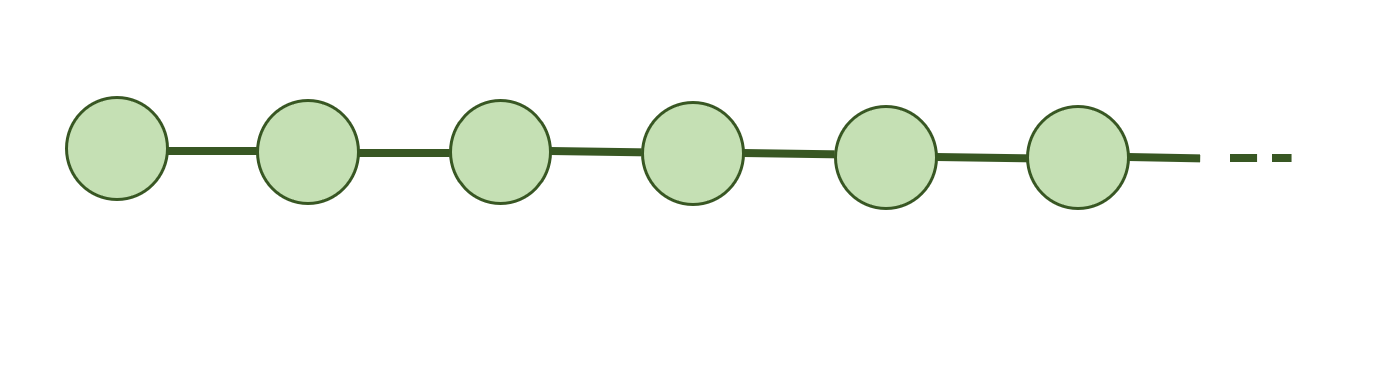
\includegraphics[width=\textwidth]{Pictures/Kontrollfragen.PNG}
        \caption{Gregory's Graph}
        \label{fig:Gregory}
    \end{figure}
\end{enumerate}

\paragraph{Aufgabe \ref{aufgabe_abstand_ex}}
Der Abstand zwischen \textbf{A} und \textbf{F} ist \(3\). Zwischen diesen Knoten gibt es die Pfade \textbf{ABEF}, \textbf{ACBEF} und \textbf{ACDEF}; der kürzeste Pfad hat Länge \(3\).
\begin{figure}[H]
    \centering
    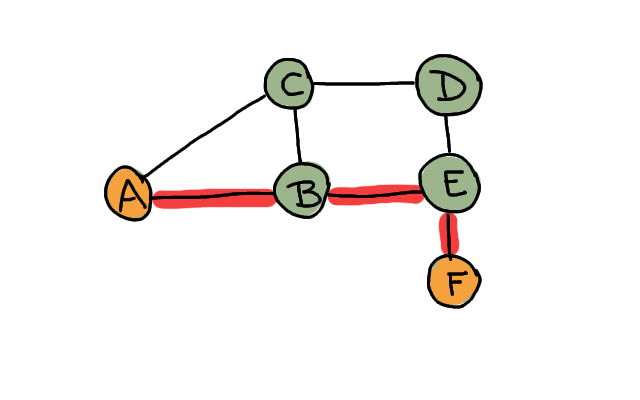
\includegraphics[width=0.5\textwidth]{Pictures/SP/abstand_ex-l1.png}
\end{figure}
Der Abstand zwischen \textbf{C} und \textbf{E} ist \(2\). Zwischen diesen Knoten gibt es die Pfade \textbf{CBE} und \textbf{CDE}. Beide haben Länge \(2\).
\begin{figure}[H]
    \centering
    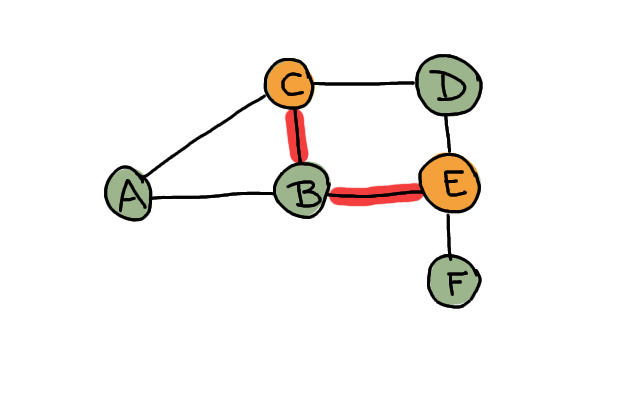
\includegraphics[width=0.5\textwidth]{Pictures/SP/abstand_ex-l2.png}
\end{figure}

\paragraph{Aufgabe \ref{aufgabe_abstand}}
\begin{enumerate}[(a)]
\item Der vollständige Graph mit 5 Knoten hat eine Kante zwischen jedem Paar von Knoten. Da jeder Knoten mit jedem anderen direkt verbunden ist, ist der Abstand zwischen zwei beliebigen Knoten \(1\).
\begin{figure}[H]
    \centering
    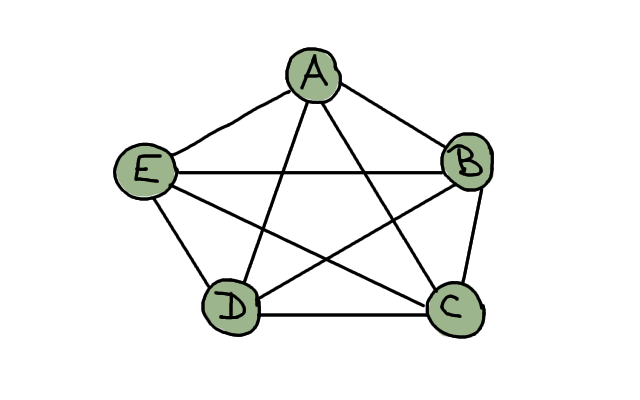
\includegraphics[width=0.5\textwidth]{Pictures/SP/abstand_k5.png}
\end{figure}

\item In einem 2 mal 3 Gittergraphen die Knoten sind in 2 Reihen und 3 Spalten organisiert und jeder Knoten ist mit den linken, rechten, oberen und unteren Nachbarn verbunden. Die zwei Knoten, die am weitesten auseinander liegen, sind die zwei diagonal zueinander stehende Ecken. Der Weg zwischen zwei solchen Ecken liegt durch die ganze Breite und die ganze Höhe des Gitters. In diesem Fall der maximale Abstand ist \(3\).
\begin{figure}[H]
    \centering
    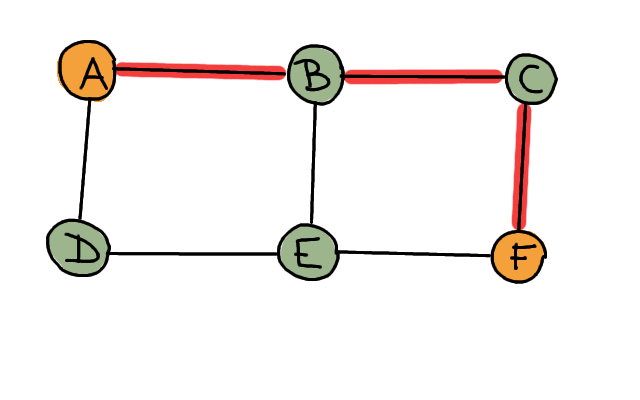
\includegraphics[width=0.5\textwidth]{Pictures/SP/abstand_gitter23.png}
\end{figure}

\item In einem Kreis gibt es zwei Pfade zwischen zwei beliebige Knoten. Zum Beispiel, zwischen \textbf{A} und \textbf{F} haben wir die Pfade \textbf{ABCDEF} und \textbf{AF}. Damit der kürzeste Pfad am Längsten wird, müssen diese zwei Pfade ungefähr gleich lang sein. Die zwei Knoten, die am weitesten ausenander sind, sind also gegenüberliegend.
\begin{figure}[H]
    \centering
    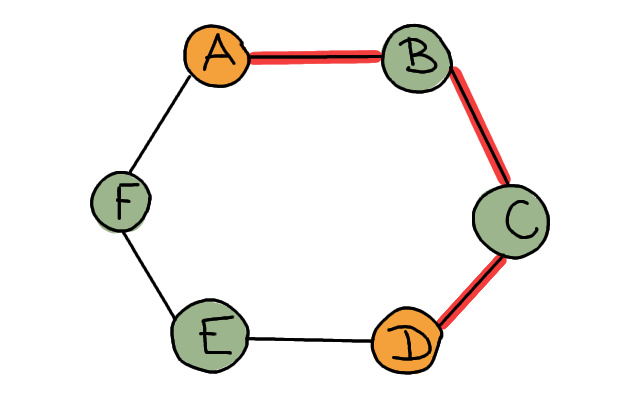
\includegraphics[width=0.5\textwidth]{Pictures/SP/abstand_kreis6.png}
\end{figure}
\end{enumerate}

\paragraph{Augabe \ref{aufgabe_panda_gebissen}}
\begin{enumerate}[(a)]
\item Die Knoten sind die genannten Leuten (Alice, Bob, Charlie, David, Elisabeth, Fred, Gregory, Hannah, Jakob, Lucy). Zwischen zwei Knoten gibt es eine Kante, wenn die entsprechenden Leuten sich irgendwoher schon kennen. Der Graph sieht dann so aus (wenn wir die Knoten mit dem ersten Buchstaben des Vornamens beschriften). Der Graph ist ungerichtet, weil wenn Person A Person B kennt, dann kennt Person B Person A auch.
    \begin{figure}[H]
        \centering
        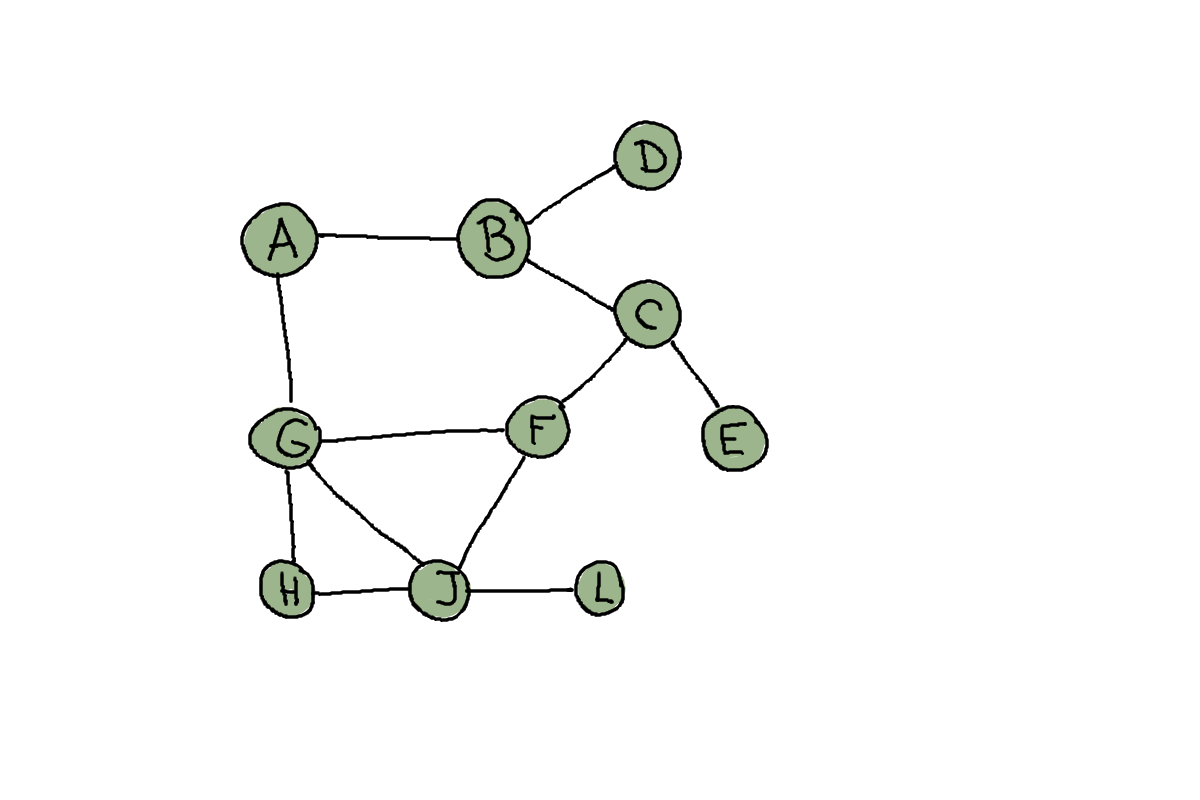
\includegraphics[width=\textwidth]{Pictures/SP/panda_gebissen_graph.png}
        \caption{Freundschaftsgraph}
        \label{fig:Gregory}
    \end{figure}

\item Wir markieren in grau die Knoten, die schon besucht worden sind und in Orange diejenigen, die sich in der Warteschlange befinden. In der Warteschlange schreiben wir unter dem Knoten auch den Abstand vom Startknoten auf.
\begin{figure}[H]
    \centering
    \begin{subfigure}[h]{0.45\textwidth}
    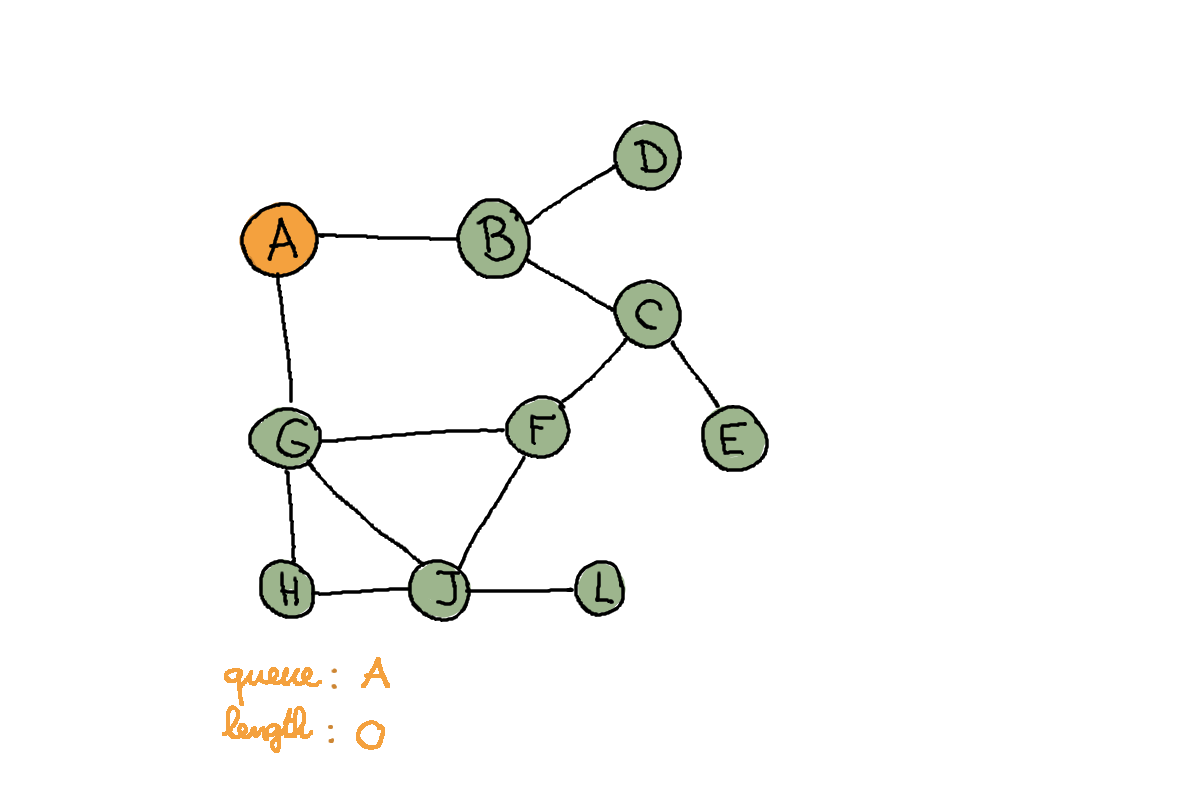
\includegraphics[width=\textwidth]{Pictures/SP/panda_gebissen_0.png}
    \end{subfigure}
    \vspace{5mm}
    \qquad
    \begin{subfigure}[h]{0.45\textwidth}
    \raggedleft
    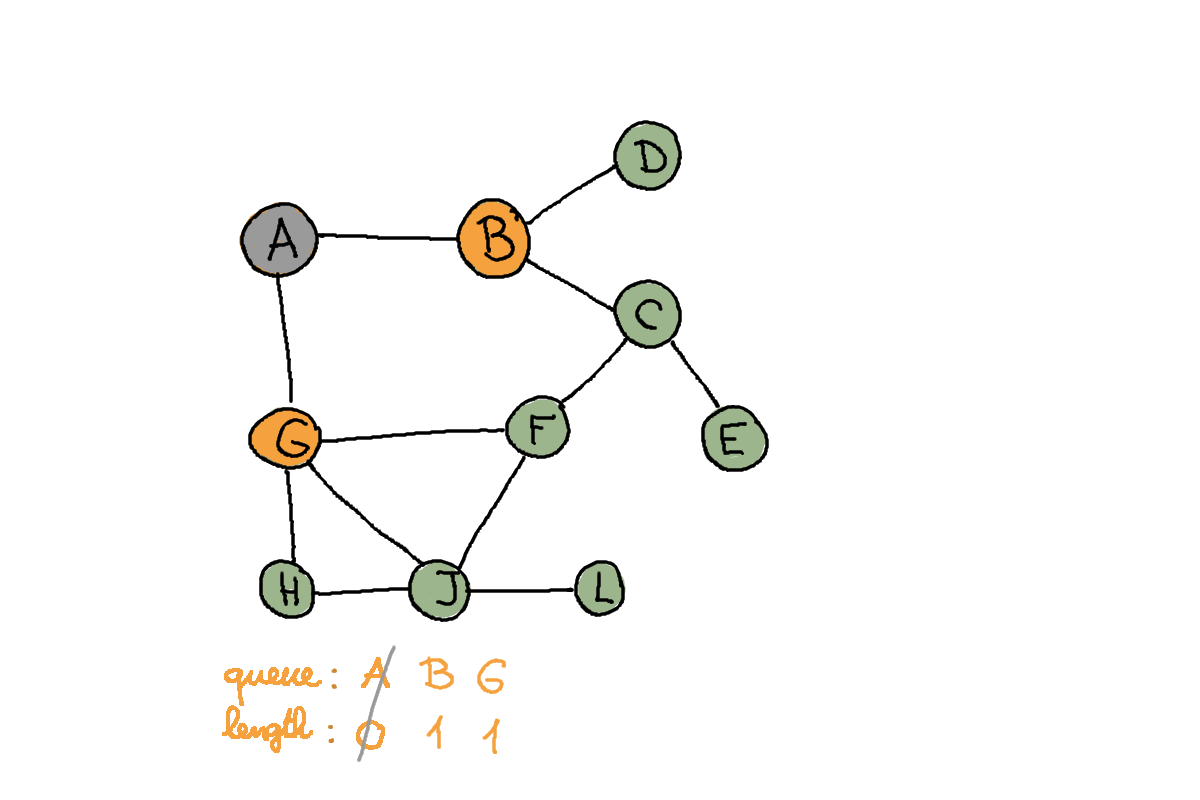
\includegraphics[width=\textwidth]{Pictures/SP/panda_gebissen_1.png}
    \end{subfigure}
    \vspace{5mm}
    \centering
    \begin{subfigure}[h]{0.45\textwidth}
    \raggedright
    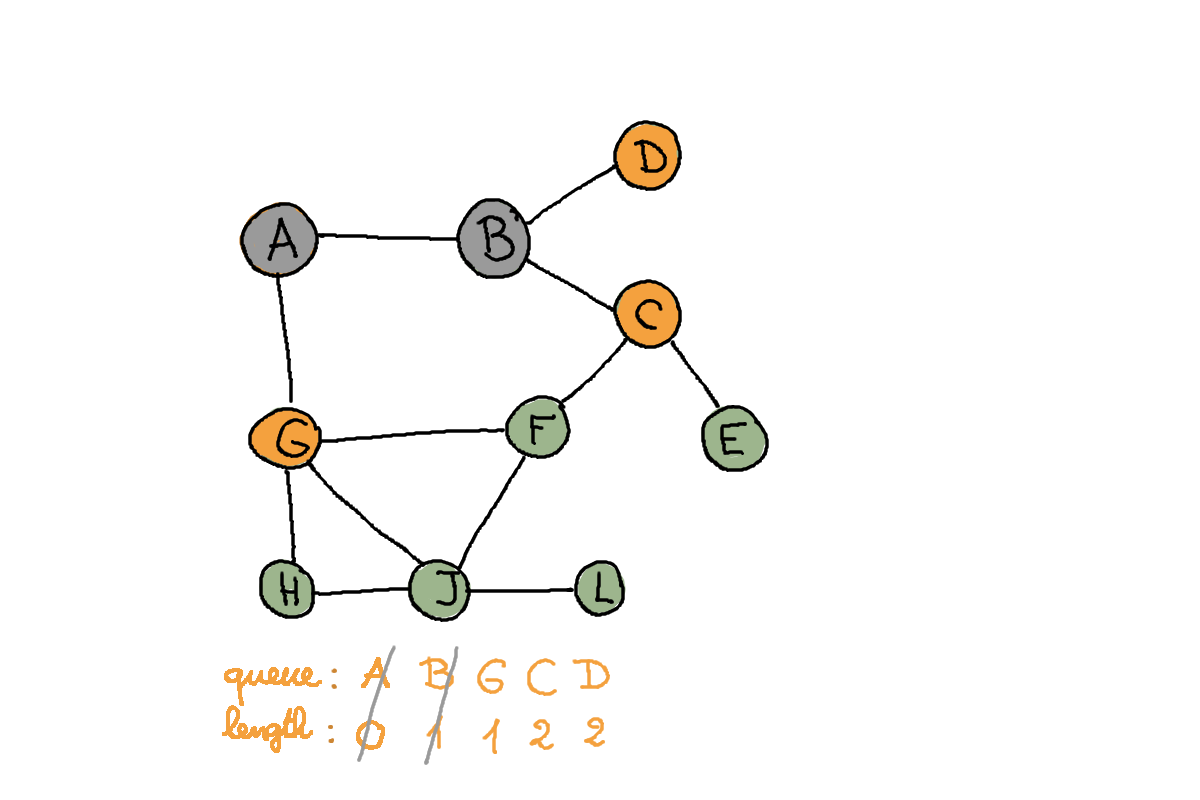
\includegraphics[width=\textwidth]{Pictures/SP/panda_gebissen_2.png}
    \end{subfigure}
    \qquad
    \begin{subfigure}[h]{0.45\textwidth}
    \raggedleft
    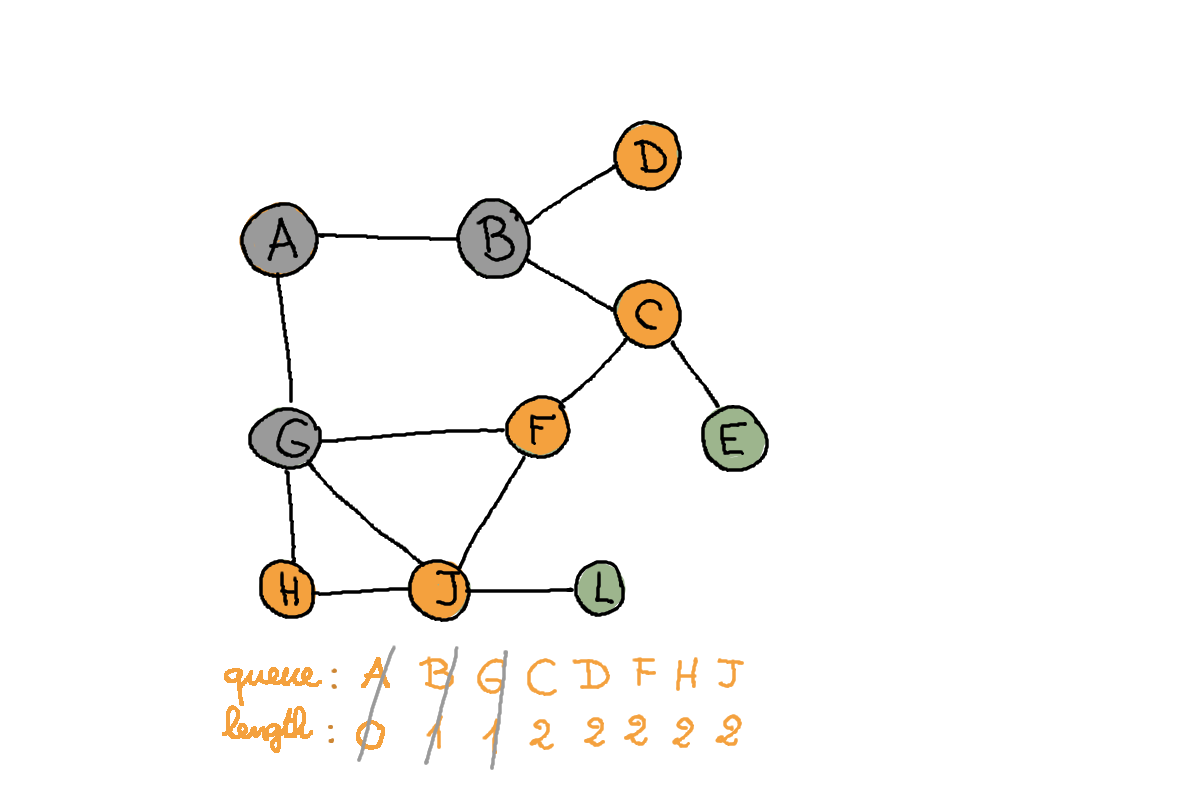
\includegraphics[width=\textwidth]{Pictures/SP/panda_gebissen_3.png}
    \end{subfigure}
\end{figure}
\begin{figure}[H]\ContinuedFloat
    \begin{subfigure}[h]{0.45\textwidth}
    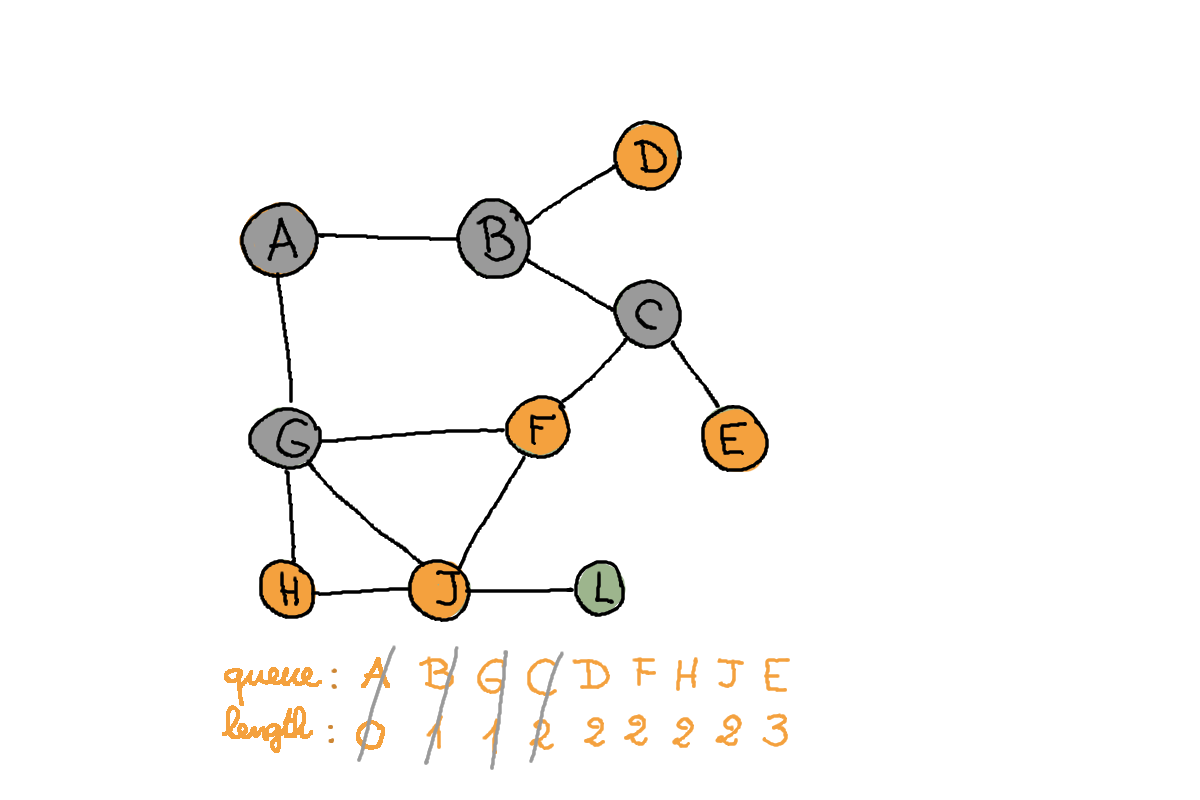
\includegraphics[width=\textwidth]{Pictures/SP/panda_gebissen_4.png}
    \end{subfigure}
    \vspace{5mm}
    \qquad
    \begin{subfigure}[h]{0.45\textwidth}
    \raggedleft
    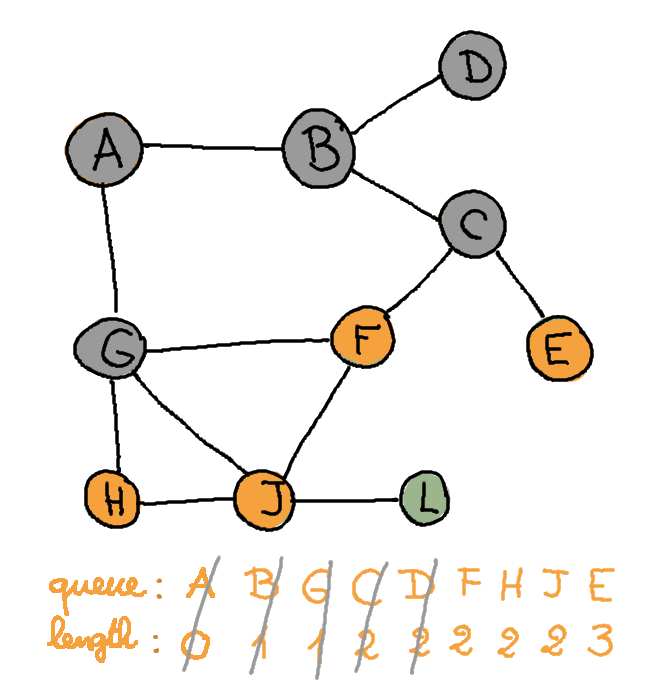
\includegraphics[width=\textwidth]{Pictures/SP/panda_gebissen_5.png}
    \end{subfigure}
    \vspace{5mm}
    \centering
    \begin{subfigure}[h]{0.45\textwidth}
    \raggedright
    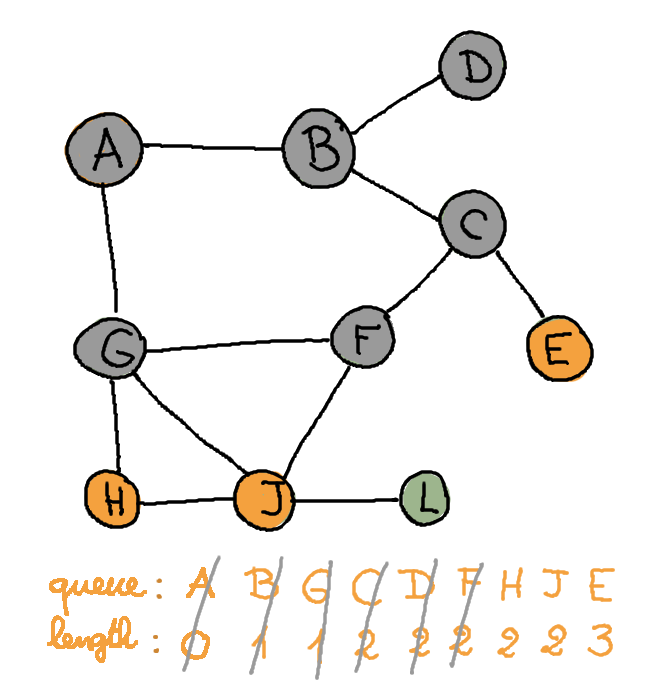
\includegraphics[width=\textwidth]{Pictures/SP/panda_gebissen_6.png}
    \end{subfigure}
    \qquad
    \begin{subfigure}[h]{0.45\textwidth}
    \raggedleft
    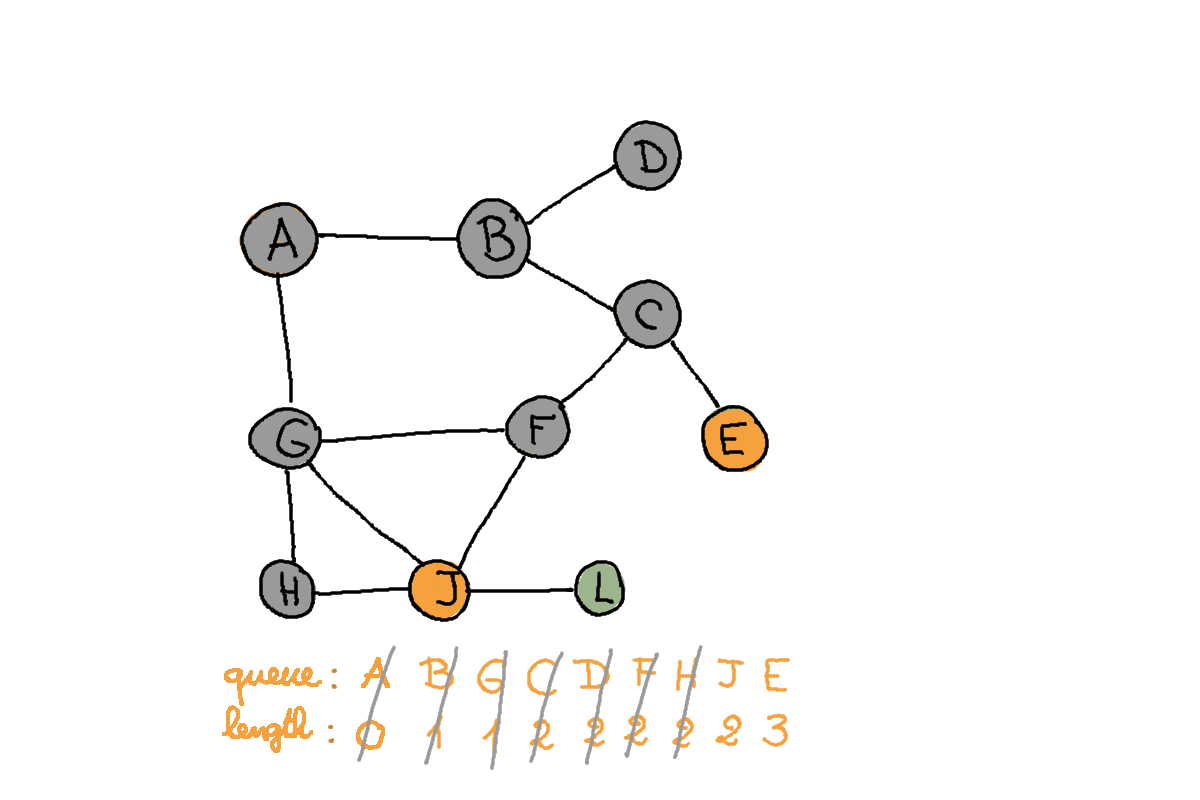
\includegraphics[width=\textwidth]{Pictures/SP/panda_gebissen_7.png}
    \end{subfigure}
\end{figure}
\begin{figure}[H]\ContinuedFloat
	\centering
    \begin{subfigure}[h]{0.6\textwidth}
    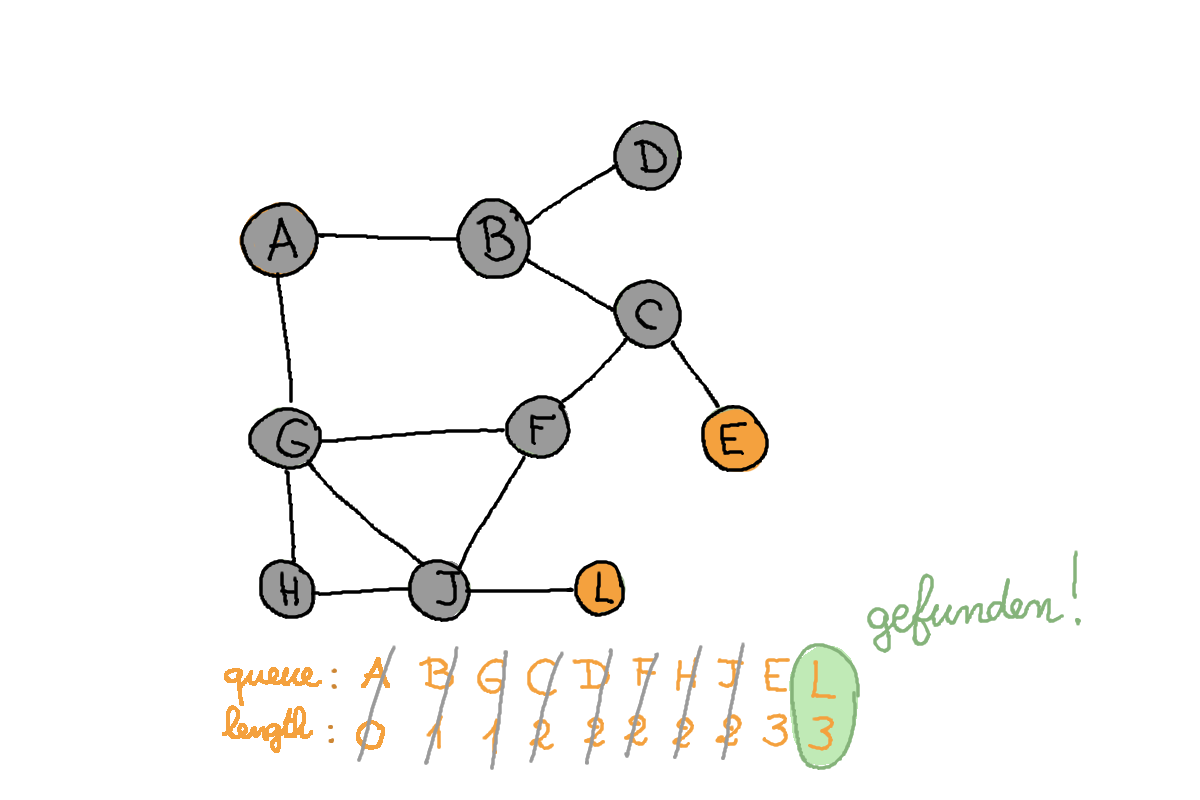
\includegraphics[width=\textwidth]{Pictures/SP/panda_gebissen_8.png}
    \end{subfigure}
\end{figure}
\item 
\begin{lstlisting}[language=Python, caption={Freundschaftsgraph in der Liste der Nachbarn Darstellung.}]
friends = {"A":["B", "G"],
        "B":["A", "C", "D"],
        "C":["B", "E", "F"],
        "D":["B"],
        "E":["C", "F"],
        "F":["C", "E", "G", "J"],
        "G":["A", "F", "H", "J"],
        "H":["G", "J"],
        "J":["F", "G", "H", "L"],
        "L":["J"]}
\end{lstlisting}
\item Dieser Graph ist klein und wir können durch Ausprobieren bestimmen, dass die zwei Knoten, die am weitesten auseinander sind, sind \textbf{D} und \textbf{L} und der Abstand zwischen diesen zwei Knoten ist \(5\).
\begin{lstlisting}[language=Python]
print(length_shortest_path(friends, "D", "L"))
5
\end{lstlisting}
Wir können aber auch ein Programm schreiben, das uns die Länge vom längsten kürzesten Pfad (den Diameter) ausrechnet. Dafür werden wir zunächst Programm \ref{lst:length_shortest_path} so umschreiben, dass es die Längen von allen kürzesten Pfaden vom Startknoten aus ausgibt. Die zwei grössten Änderungen sind, dass wir die Abstände nun auch in \texttt{visited} reinschreiben, so dass wir sie ausgeben können, und dass wir die Suche nicht mehr abbrechen, wenn wir den Endknoten gefunden haben (deswegen geben wir dem Programm auch keinen Endknoten mit).
\begin{lstlisting}[language=Python, caption={Programm, welches die Abstände vom Startknoten zu allen anderen erreichbaren Knoten ausrechnet}]
def length_all_shortest_paths_from(graph, initial):
    queue = [(initial, 0)]
    visited = {initial: 0}
    while queue:
        (node, length) = queue.pop(0)
        newlength = length + 1
        neighbours = graph[node]
        for neighbour in neighbours:
            if neighbour not in visited.keys():
                queue.append((neighbour, newlength))
                visited[neighbour] = newlength
    return visited
\end{lstlisting}
Jetzt können wir dieses Programm verwenden, um den Diameter auszurechnen. Wir gehen durch alle Knoten im Graphen durch und rufen \texttt{length\_all\_shortest\_paths\_from} auf. Das gibt uns für jeden Knoten die Abstände zu allen anderen erreichbaren Knoten im Graphen. Dann nehmen wir das Maximum über all diesen kürzesten Pfade und somit bestimmen wir den Diameter.
\begin{lstlisting}[language=Python, caption={Programm, welches den Diameter von einem Graphen bestimmt}]
def diameter(graph):
    maximum = (0, "from", "to")
    for node in graph.keys():
        all_shortest_from = length_all_shortest_paths_from(graph, node)
        farthest_from_node = max(all_shortest_from, key=all_shortest_from.get)
        if (all_shortest_from[farthest_from_node] > maximum[0]):
            maximum = (all_shortest_from[farthest_from_node], node, farthest_from_node)
    return maximum
\end{lstlisting}
Wenn wir dieses Programm ausführen, erfahren wir, dass der Diameter vom Fraundschaftsgraphen 5 ist, und dass der Abstand zwischen \texttt{D} und \texttt{L} genau diesen Wert hat.
\begin{lstlisting}[language=Python]
print(diameter(friends))
(5, 'D', 'L')
\end{lstlisting}
\end{enumerate}

\paragraph{Aufgabe \ref{aufgabe_shortest_path}}
Zuerst verwenden wir die Breitensuche, um alle Elternknoten zu ermitteln. Dann führen wir \texttt{backtracking} aus.
\begin{lstlisting}[language=Python]
def shortest_path(graph, initial, goal):
    parents = bfs_with_parent(graph, initial)
    return backtracking(parents, goal)
\end{lstlisting}

\paragraph{Aufgabe \ref{aufgabe_erde_mars_graph}}
\begin{enumerate}[(a)]
    \item Die Knoten sind die Wörter aus der Liste. Es gibt genau dann eine Kante zwischen zwei Wörter, wenn die Wörter sich um genau einen Buchstaben unterscheiden, wie zum Beispiel \texttt{MARS} und \texttt{MARK}. Der Graph ist ungerichtet, weil wenn sich ein Wort A um einen Buchstaben von einem Wort B unterscheidet, dann unterscheidet sich auch Wort B vom Wort A um einen Buchstaben.
    
    \item Der Graph sieht fol­gen­der­ma­ssen aus:
    \begin{figure}[H]
    \centering
    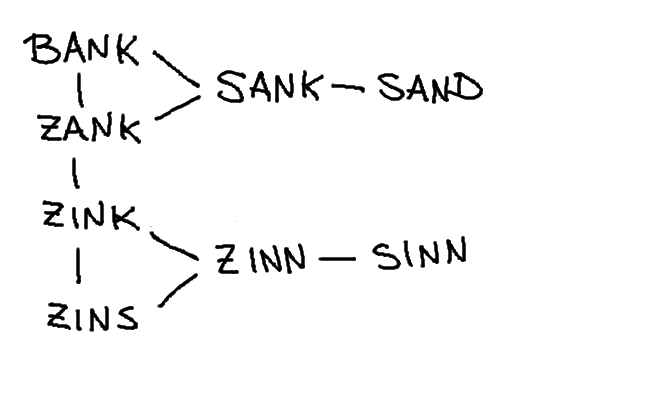
\includegraphics[width=0.6\textwidth]{Pictures/SP/bank_zins.png}
\end{figure}

	\item Ja, der Pfad ist
	\begin{lstlisting}
BANK - ZANK - ZINK - ZINS.
	\end{lstlisting}
	
	\item Ja, es reicht sogar ein Wort: \texttt{SIND}. Dann der Pfad wäre
	\begin{lstlisting}
BANK - SANK - SAND - SIND - SINN - ZINN - ZINS.
	\end{lstlisting}
	\begin{figure}[H]
    \centering
    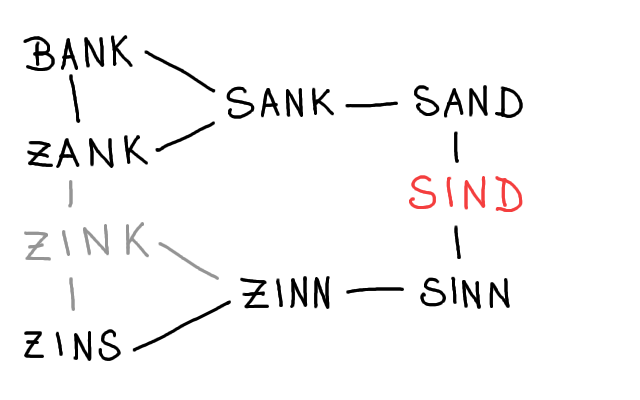
\includegraphics[width=0.6\textwidth]{Pictures/SP/bank_zins_sind.png}
\end{figure}	
\end{enumerate}

\paragraph{Aufgabe \ref{aufgabe_erde_mars_neighbours}}
\begin{enumerate}[(a)]
    \item
    \begin{lstlisting}[language=Python]
words = {"ERDE":["EIDE", "ENDE", "ERLE"],
    "EIDE":["EILE", "EINE", "ENDE", "ERDE"],
    "EINE":["EIDE", "EILE", "EINS"],
    "EINS":["EINE", "PINS", "ZINS"],
    "ZINS":["EINS", "PINS", "ZINK", "ZINN"],
    "ZINK":["ZINS", "ZINN", "ZANK", "ZICK"],
    "ZANK":["BANK", "SANK", "ZACK", "ZINK"],
    "ZACK":["ZANK", "PACK", "ZICK", "SACK"],
    "PACK":["ZACK", "SACK", "PARK"],
    "PARK":["PACK", "PARD", "MARK"],
    "MARK":["PARK", "MARS"],
    "MARS":["MARK", "MAUS"],
    "MAUS":["MARS", "HAUS"],
    "HAUS":["MAUS", "HASS"],
    "HASS":["HAUS", "BASS"],
    "BASS":["HASS"],
    "PARD":["PARK"],
    "BAND":["SAND", "BANK"],
    "SAND":["BAND", "SANK"],
    "SACK":["SANK", "ZACK", "PACK"],
    "BANK":["BAND", "SANK", "ZANK"],
    "SANK":["BANK", "ZANK", "SACK", "SAND"],
    "SINN":["ZINN"],
    "ZINN":["SINN", "ZINK", "ZINS"],
    "ZICK":["ZINK", "ZACK"],
    "PINS":["ZINS","EINS"],
    "EILT":["EILE"],
    "EILE":["EINE", "EILT", "EULE"],
    "EULE":["EILE", "ERLE"],
    "ERLE":["EULE", "ERDE"],
    "ENDE":["ERDE", "EIDE", "ENTE"],
    "ENTE":["ENDE"]}
    \end{lstlisting}
    
    \item
    \begin{lstlisting}[language=Python]
print(shortest_path(words, "ERDE", "MARS"))
['ERDE', 'EIDE', 'EINE', 'EINS', 'ZINS', 'ZINK', 'ZANK', 'ZACK', 'PACK', 'PARK', 'MARK', 'MARS']
    \end{lstlisting}
    
    \item Die Idee ist, dass wir zuerst für den ersten Buchstaben alle 26 Möglichkeiten ausprobieren. Wenn wir auf dieser Art und Weise ein Wort aus der Referenzliste kriegen, dann fügen wir es zu den Nachbarn hinzu. Mit dem zweiten, dritten und vierten Buchstaben gehen wir analog vor.
    \begin{lstlisting}[language=Python]
def compute_neighbours(nodes, node):
    neighbours = []
    for c1 in string.ascii_uppercase:
        neighbour = c1+node[1:4]
        if neighbour != node:
            if neighbour in nodes:
                neighbours.append(neighbour)
                
    for c2 in string.ascii_uppercase:
        neighbour = node[0]+c2+node[2:4]
        if neighbour != node:
            if neighbour in nodes:
                neighbours.append(neighbour)
    
    for c3 in string.ascii_uppercase:
        neighbour = node[0:2]+c3+node[3:4]
        if neighbour != node:
            if neighbour in nodes:
                neighbours.append(neighbour)
                
    for c4 in string.ascii_uppercase:
        neighbour = node[0:3]+c4
        if neighbour != node:
            if neighbour in nodes:
                neighbours.append(neighbour)
    return neighbours
    \end{lstlisting}
    Dieses Programm kann eleganter gemacht werden, indem man eine Schleife anstatt von den vier ähnlichen Blöcke verwendet.
    
    \item Das Programm, welches den kürzesten Pfad berechnet, ruft zwei Programme auf: \texttt{bfs\_with\_parent} und \texttt{backtracking}. In \texttt{bfs\_with\_parent} haben wir die nicht besuchten Nachbarn aus dem Graphen in der Liste der Nachbarn Darstellung einfach ablesen können. Nun werden wir aber nur die Liste aller Knoten (auch Referenzliste in der vorherigen Teilaufgabe genannt) herumreichen. Die Nachbarn eines Knotens müssen wir also mit \texttt{compute\_neighbours} (siehe vorherige Teilaufgabe) berechnen. Das \texttt{backtracking} Programm bleibt hingegen unverändert.
    \begin{lstlisting}[language=Python]
def bfs_with_parent_neighbours(nodes, initial):
    queue = [initial]
    visited = {initial:None}
    while queue:
        node = queue.pop(0)
        neighbours = compute_neighbours(nodes, node)
        for neighbour in neighbours:
            if neighbour not in visited:
                queue.append(neighbour)
                visited[neighbour] = node
    return visited
    
def shortest_path_neighbours(nodes, initial, goal):
    parents = bfs_with_parent_neighbours(nodes, initial)
    return backtracking(parents, goal)
    \end{lstlisting}  
\end{enumerate}

\paragraph{Aufgabe \ref{aufgabe_schlangenspiel}}
\begin{enumerate}[(a)]
    \item Die Knoten sind die Kästchen, wo die Zahlen stehen. Zwischen Knoten A und Knoten B gibt es eine Kante, wenn Kästchen B aus dem Kästchen A mit einem Würfelwurf erreicht werden kann (inklusive Schlagen- und Leiterzauber). Der Graph ist gerichtet, weil man nicht zurück oder in der Gegenrichtung von Zauberkästchen gehen kann.
    \item Eine mögliche Darstellung ist:
    \begin{lstlisting}[language=Python]
snakes_and_ladders = {
    0: [1, 3, 5, 11],
    1: [3, 5, 11],
    2: [3, 5, 6, 11],
    3: [1, 5, 6, 11],
    4: [1, 5, 6, 8],
    5: [1, 6, 8, 9],
    6: [1, 3, 8, 9],
    7: [3, 8, 9, 11],
    8: [3, 9, 11],
    9: [3, 11],
    10: [11],
    11: []
}
    \end{lstlisting}
    
    \item
    \begin{lstlisting}[language=Python]
print(shortest_path(snakes_and_ladders, 0, 11))
[0, 11]
    \end{lstlisting}
    Bob muss eine 4 Würfeln, dann hat er beim ersten Wurf gewonnen.
    
    \item Wir können die Liste der Nachbarn so umschreiben, dass wir die gewürfelte Zahl mitgeben. Dann können wir diese Zahl als Teil vom Nachbarn herumreichen.
    \item Wir brauchen zusätzlich ein Wörterbuch, welches die Zauberfelder (Schlangen und Leiter) auf die effektiven Felder übersetzt. Auf dem kleinen Spielfeld würde das Wörterbuch so aussehen.
    \begin{lstlisting}[language=Python]
magic_squares = {
    2: 5,
    4: 11,
    7: 1,
    10: 3
}
    \end{lstlisting}
    Um die Nachbarn zu ermitteln, addieren wir die gewürfelte Zahl und dann übersetzen wir sie mit dem Wörterbuch, um ''Zauberfelber'' richtig zu behandeln.
    
    Wir müssen jetzt bestimmen, was passiert, wenn man eine zu hohe Zahl würfelt. Das einfachste ist den Spieler in einem solchen Fall gewinnen zu lassen. Dafür mussen wir noch ein paar ''Zauberfelder'' einfügen.
    \begin{lstlisting}[language=Python]
magic_squares = {
    2: 5,
    4: 11,
    7: 1,
    10: 3,
    12: 11,
    13: 11,
    14: 11,
    15: 11
}
    \end{lstlisting}
    Dieses Programm gibt manche Nachbarn doppelt aus, aber bei der Breitensuche, wo wir den \texttt{visited}-Vektor haben, wird es keinen Effekt auf die Korrektheit haben.
    \begin{lstlisting}[language=Python]
def compute_neighbours(magic_dict, node):
    neighbours = []
    for i in [1, 2, 3, 4]:
        neighbour = node + i
        if neighbour in magic_dict.keys():
            neighbour = magic_dict[neighbour]
        neighbours.append(neighbour)
    return neighbours
    \end{lstlisting}{}
    
    \item Zuerst modifizieren wir \texttt{compute\_neighbours} so, dass wir nicht nur die Nachbarn berechnen sondern auch die gewürfelten Zahlen nicht verlieren.
    \begin{lstlisting}[language=Python]
def compute_neighbours_and_dice(magic_dict, node):
    neighbours = []
    for i in [1, 2, 3, 4]:
        neighbour = node + i
        if neighbour in magic_dict.keys():
            neighbour = magic_dict[neighbour]
        neighbours.append((neighbour, i))
    return neighbours
    \end{lstlisting}
    
    Dann schreiben wir \texttt{bfs\_with\_parent} um, so dass wir die gewürfelten Zahlen nicht verlieren.
    \begin{lstlisting}
def bfs_with_parent_and_dice(magic_dict, initial):
    queue = [initial]
    visited = {initial:(None, None)}
    while queue:
        node = queue.pop(0)
        neighbours_and_die = compute_neighbours_and_dice(magic_dict, node)
        for (neighbour, dice) in neighbours_and_die:
            if neighbour not in visited:
                queue.append(neighbour)
                visited[neighbour] = (node, dice)
    return visited
    \end{lstlisting}
    
    Dieses Mal müssen wir das \texttt{backtracking} Programm umschreiben, weil wir anstatt von den Knoten die gewürfelten Zahlen ausgeben wollen.
    \begin{lstlisting}[language=Python]
def backtracking_dice(parents_and_dice, goal):
    reversed_path = []
    (node, dice) = parents_and_dice[goal]
    while node != None:
        reversed_path.append(dice)
        (node, dice) = parents_and_dice[node]
    return list(reversed(reversed_path))
    \end{lstlisting}
    
    Jetzt können wir wie gewohnt alle Teile zusammensetzen.
    \begin{lstlisting}[language=Python]
def shortest_path_neighbours_and_dice(magic_dict, initial, goal):
    parents_and_dice = bfs_with_parent_and_dice(magic_dict, initial)
    return backtracking_dice(parents_and_dice, goal)
    \end{lstlisting}
    
    Wir sind endlich bereit, das grosse Schlangenspiel zu lösen.
    \begin{lstlisting}[language=Python]
magic_squares_big = {
    39: 2,
    15: 5,
    17: 22,
    14: 35,
    56: 36,
    42: 55,
    26: 45,
    32: 13,
    9: 11,
    51: 30,
    60: 59,
    61: 59,
    62: 59,
    63: 59,
}

print(shortest_path_neighbours_and_dice(magic_squares_big, 0, 59))
[1, 4, 4, 3, 3, 4, 4]
    \end{lstlisting}
    Es ist möglich, das grosse Schlangenspiel in 7 Würfe zu gewinnen, wenn man jedes Mal die richtige Zahl würfelt.
\end{enumerate}










